\documentclass[12pt]{article}
\usepackage{amsbsy,amsmath,amsthm,amssymb,subcaption}
\usepackage{graphicx}
\usepackage{enumerate}
\usepackage{natbib}
\usepackage{url} % not crucial - just used below for the URL 
\usepackage{hyperref}
\usepackage{bm}
\usepackage{xr}
\externaldocument{RJMCMC-r2}
\usepackage{alphalph}
\usepackage{xcolor}

%\pdfminorversion=4
% NOTE: To produce blinded version, replace "0" with "1" below.
\newcommand{\blind}{1}

\makeatletter
\def\namedlabel#1#2{\begingroup
	#2%
	\def\@currentlabel{#2}%
	\phantomsection\label{#1}\endgroup
}
\makeatother

\newcommand{\df}{\mathrm{d}}
\newcommand{\X}{\mathsf{X}}
\newcommand{\Y}{\mathsf{Y}}
\newcommand{\Z}{\mathsf{Z}}
\newcommand{\SF}{\mathcal{A}}
\newcommand{\A}{\mathcal{A}}
\newcommand{\F}{\mathcal{F}}
\newcommand{\Par}{\X}
\newcommand{\Q}{\hat{Q}}
\newcommand{\prior}{m^{\scriptsize\mbox{pr}}}
\newcommand{\Prior}{M^{\scriptsize\mbox{pr}}}
\newcommand{\pprior}{p^{\scriptsize\mbox{pr}}}
\newcommand{\ind}{\mathbf{1}}
\newcommand{\Mtk}{\mtkfont{T}}
\newcommand{\mtkfont}{\mathcal}
\newcommand{\pcite}[1]{\citeauthor{#1}'s \citeyearpar{#1}}

\newtheorem{theorem}{Theorem}
\newtheorem{lemma}[theorem]{Lemma}
\newtheorem{corollary}[theorem]{Corollary}
\newtheorem{proposition}[theorem]{Proposition}
\newtheorem{definition}[theorem]{Definition}
\newtheorem{assumption}[theorem]{Assumption}
\newtheorem{example}[theorem]{Example}
\newtheorem{remark}[theorem]{Remark}

% DON'T change margins - should be 1 inch all around.
\addtolength{\oddsidemargin}{-.5in}%
\addtolength{\evensidemargin}{-1in}%
\addtolength{\textwidth}{1in}%
\addtolength{\textheight}{1.7in}%
\addtolength{\topmargin}{-1in}%




\begin{document}
	
	%\bibliographystyle{natbib}
	
	\def\spacingset#1{\renewcommand{\baselinestretch}%
		{#1}\small\normalsize} \spacingset{1}
	
	
	%%%%%%%%%%%%%%%%%%%%%%%%%%%%%%%%%%%%%%%%%%%%%%%%%%%%%%%%%%%%%%%%%%%%%%%%%%%%%%
	
	\if1\blind
	{
		\title{\bf Supplement II: Autoregression with Laplace errors}
		\author{}
		\maketitle
	} \fi
	
	\if0\blind
	{
		\title{\bf Supplement II: Autoregression with Laplace errors}
		\author{Qian Qin\thanks{
				Partially supported by NSF DMS-2112887}\hspace{.2cm}\\
			School of Statistics, University of Minnesota}
		\maketitle
	} \fi

	\maketitle
	
	\spacingset{1.9} % DON'T change the spacing!
	
	
	
	\renewcommand*{\thetheorem}{\alph{theorem}}
	\def\theequation{\alphalph{\value{equation}}}
	\def\thefigure{\alphalph{\value{figure}}}
	\def\thetable{\alphalph{\value{table}}}
	\def\thesection{\alphalph{\value{section}}}
	
	Bayesian autoregression with an unknown model order is a scenario where trans-dimensional MCMC naturally applies.
	See \cite{troughton1998reversible}, \cite{ehlers2002efficient}, \cite{vermaak2004reversible}.
	Consider a Bayesian autoregression with Laplace errors.
	This model is practically relevant for its use in Bayesian quantile regression \citep{yu2001bayesian}.
	
	
	\section{The model}
	
	
	
	
	Suppose that $Y_i \in \mathbb{R}$ and $x_i \in \mathbb{R}^p$ satisfy, for $i = 1, \dots, n$, 
	\[
	Y_i = \sum_{j=1}^K A_j Y_{i-j} + x_i^{\top} B + \sqrt{T} E_i,
	\]
	where $E_1, \dots, E_n$ are iid random errors with a Laplace density $f_E(\epsilon) = e^{-|\epsilon|/2}/4$, $K$~is the unknown model order, $A_1, \dots, A_K$ are unknown autoregression coefficients,~$B$ is an unknown $p$-dimensional regression coefficient, and~$T$ is an unknown dispersion parameter.
	If $K = 0$, the summation from $j = 1$ to~$K$ is interpreted as zero.
	The predictors $(x_i)_{i=1}^n$ are known, while the responses $(Y_i)_{i=1}^n$ are observable.
	To ensure that the model is well-specified, assume that $(Y_i)_{i=1}^n$ has a known starting sequence, $(Y_i)_{i=-k_{\scriptsize \mbox{max}} + 1}^0 = (y_i)_{i=-k_{\scriptsize \mbox{max}} + 1}^0$, where $k_{\scriptsize \mbox{max}}$ is a positive integer.
	The goal is to make inference about the parameters~$K$, $(A_j)_{j=1}^K$,~$B$, and~$T$.
	
	
	
	
	
	Let $Y = (Y_1, \dots, Y_n)^{\top} \in \mathbb{R}^n$ and $A = (A_1, \dots, A_K)^{\top} \in \mathbb{R}^K$.
	Given $(K,A,B,T) = (k,\alpha, \beta, \tau)$, the likelihood of~$Y$ evaluated at $y = (y_1, \dots, y_n)^{\top}$ is
	\[
	f(y \mid k, \alpha, \beta, \tau) = \frac{1}{4^n \tau^{n/2}} \exp \left( - \frac{1}{2\sqrt{\tau}} \sum_{i=1}^n \left|y_i - x_i^{\top} \beta - w_{i,k}^{\top} \alpha \right| \right),
	\] 
	where  $w_{i,k} = (y_{i-1}, \dots, y_{i-k})^{\top}$ for $i = 1,\dots,n$.
	
	
	
	To perform Bayesian analysis, place a prior density on $(K,A,B,T)$ of the form
	\[
	f_K(k) \, f_A(\alpha \mid k, \tau)^{\ind_{\{0\}^c}(k)} f_B(\beta \mid \tau) f_T(\tau).
	\]
	To be precise, $f_K$ is an arbitrary probability mass function that is positive on $\mathsf{K}= \{0, \dots, k_{\scriptsize \mbox{max}}\};$ 
	$f_A(\cdot \mid k, \tau)$ is the density of the $\mbox{N}_k(0, \sigma^2 \tau I_k)$ distribution, where~$\sigma$ is a positive hyperparameter, and $I_k$ is the $k \times k$ identity matrix;
	$f_B(\beta \mid \tau)$ is the density of the $\mbox{N}_p(0, \sigma^2 \tau I_p)$ distribution;
	$f_T(\tau)$ is proportional to $\tau^{-1}$.
	The resultant (un-normalized) posterior density is
	\[
	\tilde{\pi}(k, \alpha, \beta, \tau \mid y) = f(y \mid k, \alpha,\beta,\tau) f_K(k) \, f_A(\alpha \mid k, \tau)^{\ind_{\{0\}^c}(k)} f_B(\beta \mid \tau) f_T(\tau).
	\]
	The posterior distribution (if proper) is intractable even when~$k$ is given.
	To facilitate sampling, we follow \cite{liu1996bayesian} and \cite{choi2013analysis}, and introduce a sequence of auxiliary random variables $U = (U_1, \dots, U_n)^{\top}$.
	Given $(K,A,B,T,Y) = (k, \alpha, \beta, \tau,y)$, the conditional distribution of~$U$ is a product of inverse Gaussian distributions, with density function
	\[
	\begin{aligned}
		&f_{U \mid \cdot}(u \mid k, \alpha, \beta, \tau, y) \\
		=& \prod_{i=1}^n \left\{ \frac{1}{\sqrt{8\bm{\pi} u_i^3}} \exp \left[ -  \frac{u_i (y_i - x_i^{\top} \beta - w_{i,k}^{\top} \alpha )^2}{2\tau} + \frac{|y_i - x_i^{\top} \beta - w_{i,k}^{\top} \alpha|}{2\sqrt{\tau}}  - \frac{1}{8u_i} \right]  \, \ind_{(0,\infty)}(u_i) \right\},
	\end{aligned}
	\]
	where $u = (u_1, \dots, u_n)^{\top}$, and $\bm{\pi}$ denotes the ratio of a circle's circumference to its diameter, not to be confused with the density function~$\pi$ defined below.
	Consider the augmented posterior density of $(K, A, B, T, U)$, given by
	\[
	\pi(k,\alpha,\beta,\tau,u \mid y) = f_{U \mid \cdot}(u \mid k, \alpha, \beta, \tau, y) \, \tilde{\pi}(k, \alpha, \beta, \tau \mid y),
	\]
	where the argument $(k, \alpha, \beta, \tau, u)$ can take values in $\bigcup_{k \in \mathsf{K}} \{k\} \times \Z_k$, with $\Z_k = \mathbb{R}^k \times \mathbb{R}^p \times (0,\infty) \times (0,\infty)^n$.
	The corresponding measure~$\Pi$ has the form~\eqref{eq:Pi}.
	The map $(\alpha, \beta, \tau, u) \mapsto \pi(k, \alpha, \beta, \tau, u \mid y)$ gives the density of $\Psi_k$ with respect to the Lebesgue measure on $\Z_k$.
	
	
	For $k \in \mathsf{K}$, let $W(k)$ be the $n \times (p+k)$ matrix whose $i$th row is $(x_i^{\top}, w_{i,k}^{\top})$.
	In what follows, assume the following:
	\begin{enumerate}
		\item [\namedlabel{P1}{(P1)}] For $k \in \mathsf{K}$, $W(k)$ has full column rank, and~$y$ is not in the column space of $W(k)$.
	\end{enumerate}
	It can then be shown that $\Psi_k(\Z_k) < \infty$ for $k \in \mathsf{K}$, and~$\Pi$ is a proper posterior distribution.
	The introduction of the auxiliary variables $U_i$ leads to a two-component Gibbs sampler that can be used to sample from $\Phi_k$, the normalization of~$\Psi_k$. 
	In what follows, the Gibbs sampler is combined with a standard reversible jump scheme to create a trans-dimensional MCMC sampler targeting~$\Pi$.
	
	
	\section{A reversible jump MCMC algorithm} \label{sssec:autogibbs}
	
	When $K$ is known to be $k \in \mathsf{K}$, a two-component Gibbs sampler can be used to sample from $\Phi_k$ \citep{choi2013analysis}.
	When the current state is $(\alpha,\beta,\tau,u) \in \Z_k$, the sampler draws the next state $(\alpha',\beta',\tau',u')$ via the following steps:
	\begin{enumerate}
		\item Draw $u' = (u_1', \dots,u_n')$ from the conditional distribution of $U$ given $(K,A,B,T,Y) = (k, \alpha, \beta, \tau,y)$, which is associated with the density $f_{U \mid \cdot}(u' \mid k, \alpha, \beta, \tau, y)$.
		\item 
		Let $Q $ be the $n \times n$ diagonal matrix whose $i$th diagonal element is $u_i'$.
		Draw $\tau'$ from the conditional distribution of $T$ given $(K,U,Y) = (k, u', y)$, which is the inverse Gamma distribution with shape parameter $n/2$ and scale parameter
		\[
		\frac{y^{\top} Q y - y^{\top} Q W(k) [W(k)^{\top} Q W(k) + \sigma^{-2} I_{p+k}]^{-1} W(k)^{\top} Q y }{2}.
		\]
		\item 
		Draw $(\beta'^{\top}, \alpha'^{\top})^{\top}$ from the conditional distribution of $(B^{\top}, A^{\top})^{\top}$ given $(K,T,U,Y) = (k,\tau', u', y)$, which is the normal distribution
		\[
		\mbox{N}_{p+k} \left( [W(k)^{\top} Q W(k) + \sigma^{-2} I_{p+k}]^{-1} W(k)^{\top} Q y, \, \tau [W(k)^{\top} Q W(k) + \sigma^{-2} I_{p+k}]^{-1} \right).
		\]
	\end{enumerate}
	Note that this is a Gibbs sampler with two components since the second and third steps are blocked, and can be viewed as drawing from the conditional distribution of $(A,B,T)$ given the rest.
	{ The resultant chain has $\Phi_k$ as its stationary distribution, but is not reversible with respect to $\Phi_k$.}
	
	
	Consider now a reversible jump algorithm for sampling from~$\Pi$.
	When the current state is $(k,\alpha, \beta, \tau, u)$, the algorithm randomly performs one of three move types, code-named U, B, and D.
	To be specific, the probability of choosing a move type depends on the current state only through~$k$, and these probabilities are denoted by $q_{\scriptsize\mbox{U}}(k)$, $q_{\scriptsize\mbox{B}}(k)$, and $q_{\scriptsize\mbox{D}}(k)$, respectively.
	The three move types are defined as follows:
	\begin{itemize}
		\item {\it U move}: 
		Draw $(\alpha',\beta',\tau',u')$ using one iteration of the two-component Gibbs sampler.
		Set the new state to $(k,\alpha',\beta',\tau',u')$.
		
		\item {\it B move}: 
		Draw $a_*$ from some distribution on $\mathbb{R}$ associated with a density function $g(\cdot \mid k, \alpha, \beta, \tau, u)$.
		Let $\alpha' = (\alpha^{\top}, a_*)^{\top}$.
		With probability
		\[
		\min \left\{ 1, \frac{  \pi(k+1, \alpha', \beta, \tau, u \mid y) \, q_{\scriptsize\mbox{D}}(k+1) }{  \pi(k, \alpha, \beta, \tau, u \mid y) \, q_{\scriptsize\mbox{B}}(k) \, g(a_* \mid k, \alpha, \beta, \tau, u) } \right\},
		\]
		set the new state to $(k+1,\alpha',\beta,\tau,u)$;
		otherwise, keep the old state.
		This move is only available when $k < k_{\scriptsize \mbox{max}}$.
		\item {\it D move}: 
		Let $\alpha' = (\alpha_1, \dots, \alpha_{k-1})^{\top}$ if $\alpha = (\alpha_1, \dots, \alpha_k)^{\top}$.
		With probability
		\[
		\min \left\{ 1, \frac{  \pi(k - 1, \alpha', \beta, \tau, u \mid y) \, q_{\scriptsize\mbox{B}}(k-1) \, g(\alpha_k \mid k - 1, \alpha', \beta, \tau, u, y) }{  \pi(k, \alpha, \beta, \tau, u \mid y) \, q_{\scriptsize\mbox{D}}(k) } \right\},
		\]
		set the new state to $(k-1,\alpha', \beta, \tau, u)$;
		otherwise, keep the old state.
		This move is only available when $k > 0$.
	\end{itemize}
	
	
	
	{ The resultant trans-dimensional Markov chain has $\Pi$ as its stationary distribution, but it is not reversible.}
	
	
	
	
	
	
	\section{Convergence analysis}
	
	
	
	For $k \in \mathsf{K}$, let $P_k$ be the Mtk of the Gibbs chain targeting $\Phi_k$.
	Then the following result holds.
	
	
	
	\begin{lemma} \label{lem:robustgeo}
		Suppose that \ref{P1} holds.
		For $k \in \mathsf{K}$, $P_k$ is $\Pi$-a.e. geometrically ergodic.
	\end{lemma}
	
	The proof of this result is given in Section~\ref{app:robustgeo}.
	It utilizes the classical drift and minorization technique, and follows closely arguments in \cite{roy2010monte}.
	\cite{roy2010monte} studied the Gibbs chain when an improper prior on $(A,B)$ is used.
	The result can also be proved using the approach of \cite{choi2013analysis}, who studied the spectral properties of a Markov operator closely related to $P_k$.
	
	Combining Lemma~\ref{lem:robustgeo} and Theorem~\ref{thm:main} yields the following for the reversible jump algorithm.
	
	\begin{proposition} \label{pro:ar}
		Suppose that \ref{P1} holds.
		Suppose further that $q_{\scriptsize\mbox{U}}(k) > 0$ for $k \in \mathsf{K}$, $q_{\scriptsize\mbox{B}}(k) > 0$ for $k < k_{\scriptsize \mbox{max}}$, and $q_{\scriptsize\mbox{D}}(k) > 0$ for $k > 0$.
		Then the reversible jump chain is $L^2(\Pi)$ geometrically convergent and $\Pi$-a.e. geometrically ergodic.
	\end{proposition}
	\begin{proof}
		Apply Theorem~\ref{thm:main}.
		Let~$P$ be the Mtk of the reversible jump chain.
		For $k \in \mathsf{K}$, (i) and (iii) in \ref{H1} hold with $P_k$ defined above and $c_k = q_{\scriptsize\mbox{U}}(k)$.
		The chain associated with $P_k$ is clearly $\varphi$-irreducible.
		By Lemma~\ref{lem:robustgeo} and (ii) in Lemma~\ref{lem:Pk-convergence}, (ii) in \ref{H1} holds with $t_0 = 1$.
		
		To verify \ref{H2}, simply note that $\bar{P}(k,\{k'\})$, the average probability flow from model~$k$ to model~$k'$, is strictly positive whenever $|k'-k| \leq 1$, indicating the between-model movements are irreducible.
		(Alternatively, note that $P$ is $\Pi$-irreducible.)
		
		
		%		To verify \ref{H2}, recall how $\Gamma_P$ is defined.
		%		Let $\Gamma_P$ be the $(k_{\scriptsize \mbox{max}}+1)\times (k_{\scriptsize \mbox{max}}+1)$ matrix whose $i,j$th element, denoted by $\gamma_{i-1,j-1}$, is one if
		%		\[
		%		\int_{\Z_{i-1}} \Psi_{i-1}(\df z) P((i-1,z), \{j-1\} \times \Z_{j-1}) > 0
		%		\]
		%		and zero otherwise.
		%		Then, for $i \in \{1,\dots, k_{\scriptsize \mbox{max}}+1\}$, $\gamma_{i-1,i-2} = \gamma_{i-1,i-1} = \gamma_{i-1,i} = 1$, provided that the subscripts are not out of bounds.
		%		Then every element of $\Gamma_{P}^{k_{\scriptsize \mbox{max}}}$ is positive.
		%		Thus, \ref{H2} holds, and~$P$ is $L^2(\Pi)$ geometrically convergent.
		
		Thus, $P$ is $L^2(\Pi)$ geometrically convergent.
		By Theorem~1 of \cite{roberts2001geometric}, it is $\Pi$-a.e. geometrically ergodic.
	\end{proof}
	
	\section{A simulated example} \label{sssec:robustsimulate}
	
	We use a simple simulated example to show how geometric ergodicity allows us to take estimation uncertainty into account when performing model selection.
	A data set satisfying condition \ref{P1} with $k_{\scriptsize \mbox{max}} = 10$, $p = 50$, $n = 100$ is simulated.
	The data set is generated according to the autoregressive model with the true model order~$K$ being~4, and the true value of~$A$ being $(0.3, 0.25, 0.05, 0.05)^{\top}$.
	
	The reversible jump algorithm is applied to the simulated data set.
	The prior distribution $f_K$ is a truncated Poisson distribution.
	The density $g(\cdot \mid k, \alpha, \beta, \tau, u)$ is taken to be the conditional density function of $A_{k+1}$ given $K=k+1$, $(A_1, \dots, A_k)^{\top} = \alpha$, $B = \beta$, $T = \tau$, $U = u$, and $Y = y$.
	This corresponds to a normal distribution.
	Following Section 4.3 of \cite{green1995reversible}, probabilities of birth and death proposals are taken to be
	\[
	q_{\scriptsize\mbox{B}}(k) = \frac{1}{3} \min \left\{ 1, \frac{f_K(k+1)}{f_K(k)} \right\}, \, q_{\scriptsize\mbox{D}}(k) = \frac{1}{3} \min \left\{ 1, \frac{f_K(k-1)}{f_K(k)} \right\}.
	\]
	%	This construction was originally proposed in Section 4.3 of \cite{green1995reversible}, and ensures that
	%	\[
	%	\frac{f_K(k+1) q_{\scriptsize\mbox{D}}(k+1)}{f_K(k) q_{\scriptsize\mbox{B}}(k)} = 1.
	%	\]
	By Proposition \ref{pro:ar}, the corresponding chain is $\Pi$-a.e. geometrically ergodic.
	
	
	%	\begin{figure}
		%		\centering
		%		\begin{subfigure}[b]{0.45\textwidth}
			%			\centering
			%			\includegraphics[width=\textwidth]{traceplot-robust}
			%		\end{subfigure}
		%		\hfill
		%		\begin{subfigure}[b]{0.45\textwidth}
			%			\centering
			%			\includegraphics[width=\textwidth]{traceplot-robust-a}
			%		\end{subfigure}
		%		\caption{Left: Trace plot of $K(t)$.
			%			Right: Trace plot of the fourth component of $A(t)$.}
		%		\label{fig:varmcmc}
		%	\end{figure}
	
	\begin{figure}
		\centering
		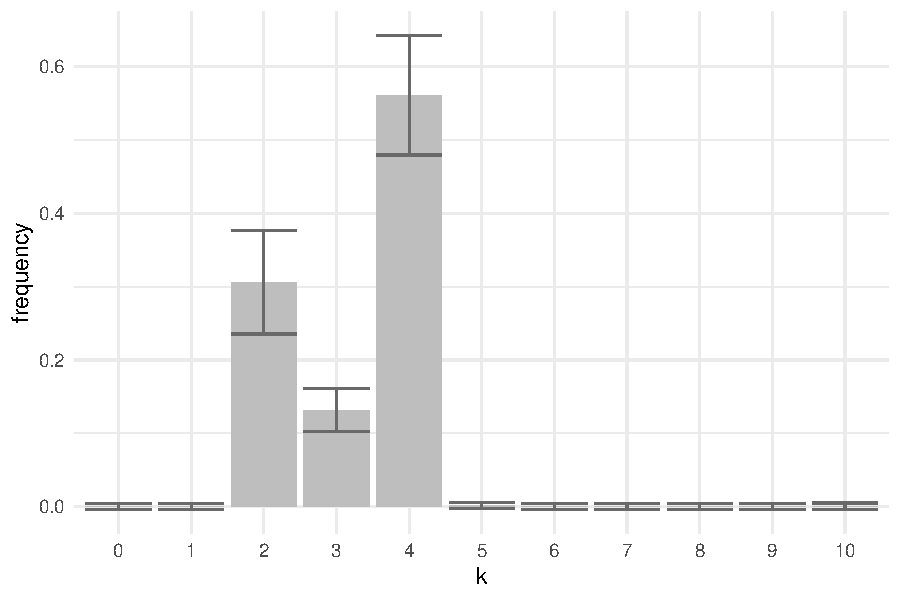
\includegraphics[width=0.7\textwidth]{robustmcmc-bonf}
		\caption{Estimated posterior distribution of $K$ with $95\%$ simultaneous confidence intervals.} \label{fig:varmcmc-2}
	\end{figure}
	
	
	
	
	%	A reversible jump chain $(K(t),Z(t))_{t \geq 0}$ is simulated, where $Z(t)$ has the form $(A(t), B(t), T(t))$.
	%	Figure \ref{fig:varmcmc} gives two trace plots.
	%	On the left, there is the trace plot of $K(t)$ for the first $1 \times 10^4$ iterations.
	%	We see that the between-model movement does not mix particularly fast, but the chain is able to move freely between two apparent modes ($k=2$ and $k=4$) given enough time.
	%	On the right, there is the trace plot of $A(t)$ for the first 1000 iterations.
	%	In the first 1000 iterations, the chain mostly stayed in models $k=3$ and $k=4$.
	%	The trace plot suggests that the within-model chain associated with $P_4$ mixes very well.
	
	Based on a simulated chain of length $m = 4 \times 10^5$, we estimate the posterior probability of $K = k$ for $k = 0,\dots,10$.
%	Under geometric ergodicity, the sample proportions are asymptotically normally distributed, and the asymptotic variances can be consistently estimated using the batch-means method \citep{jones2006fixed}.
	We construct simultaneous 95\% Wald confidence intervals for the posterior probabilities using Bonferroni correction.
	Like in Section \ref{sssec:binary-example}, we add $(\log m) \sqrt{1/b_m^2+b_m/m}$ to the estimated asymptotic variances, where $b_m \approx m^{0.6}$ is the batch size.
	The posterior probability estimates and confidence intervals are visualized in Figure \ref{fig:varmcmc-2}.
	We may thus conclude with high confidence that $K=4$ is the most favored model, while $K=2$ is in second place.
	
	
	
	%	In accordance with the discussion in Section \ref{sec:uncertainty}, a tiny amount of noise ($\varepsilon = 0.01$) has been injected into the Monte Carlo estimator.
	
	
	\section{Proof of Lemma~\ref{lem:robustgeo}} \label{app:robustgeo}
	
	Fix $k \in \mathcal{K}$.
	Suppose that $(A(t), B(t), T(t), U(t))_{t=0}^{\infty}$ is a chain associated with $P_k$.
	Then $(A(t), B(t), T(t))_{t=0}^{\infty}$ is also a Markov chain that has the same convergence rate in the total variation distance.
	This is because the two chains are co-de-initializing \citep{roberts2001markov}.
	Thus, it suffices to show that the latter is $\hat{\Phi}_k$-a.e. geometrically ergodic, where $\hat{\Phi}_k$ is the distribution of $(A,B,T)$ given $(K,Y) = (k,y)$.
	
	
	To show geometric ergodicity one can establish a set of drift and minorization conditions \citep{rosenthal1995minorization}.
	Let $\hat{P}_k$ be the Mtk of $(A(t), B(t), T(t))_{t=0}^{\infty}$.
	For $(\alpha, \beta, \tau) \in \mathbb{R}^k \times \mathbb{R}^p \times (0,\infty)$, let
	\[
	V(\alpha, \beta, \tau) = \frac{\sum_{i=1}^N (y_i - x_i^{\top} \beta - w_{i,k}^{\top} \alpha)^2}{\tau}.
	\]
	The following two lemmas establish a set of drift and minorization conditions for $\hat{P}_k$.
	Similar arguments can be found in, e.g., \cite{roy2010monte} and \cite{hobert2015convergence}.
	
	\begin{lemma} \label{lem:robustdrift}
		Assume that \ref{P1} holds.
		There exist $\lambda < 1$ and $L < \infty$ such that the following holds for each $(\alpha, \beta, \tau) \in \mathbb{R}^k \times \mathbb{R}^p \times (0,\infty)$:
		\[
		\hat{P}_k V(\alpha, \beta, \tau) \leq \lambda V(\alpha, \beta, \tau) + L.
		\]
	\end{lemma}
	
	\begin{proof}
		Fix $(\alpha, \beta, \tau) \in \mathbb{R}^k \times \mathbb{R}^p \times (0,\infty)$.
		Let $(A',B',T') \sim \hat{P}_k((\alpha, \beta, \tau), \cdot)$.
		Recalling the steps of the two-component Gibbs algorithm, one can obtain
		\[
		\begin{aligned}
			\hat{P}_k V(\alpha, \beta, \tau) =& E \left[ V(A',B',T') \right] \\
			=& E\left\{ \frac{\|y - W(k) [W(k)^{\top} Q W(k) + \sigma^{-2} I_{p+k} ]^{-1} W(k)^{\top} Q y \|^2 }{T'} \right\} + \\
			& E \left( \mbox{tr} \left\{ W(k) [W(k)^{\top} Q W(k) + \sigma^{-2} I_{p+k} ]^{-1} W(k)^{\top} \right\} \right) \\
			=& E\left\{ \frac{N \| y -  W(k) [W(k)^{\top} Q W(k) + \sigma^{-2} I_{p+k} ]^{-1} W(k)^{\top} Q y \|^2 }{ y^{\top} Q y - y^{\top} Q W(k) [W(k)^{\top} Q W(k) + \sigma^{-2} I_{p+k}]^{-1} W(k)^{\top} Q y } \right\} + \\
			& E \left( \mbox{tr} \left\{ W(k) [W(k)^{\top} Q W(k) + \sigma^{-2} I_{p+k} ]^{-1} W(k)^{\top} \right\} \right),
		\end{aligned}
		\]
		where $W(k)$ is the $N \times (p+k)$ matrix whose $i$th row is $(x_i^{\top}, w_{i,k}^{\top})$, and $Q$ is the $N \times N$ diagonal matrix whose diagonal elements $(U_1',\dots, U_N')$ are distributed according to the density 
		\[
		\begin{aligned}
			&f_{U \mid \cdot}(u' \mid k, \alpha, \beta, \tau, y) \\
			=& \prod_{i=1}^N \left\{ \frac{1}{\sqrt{8\bm{\pi} u_i'^3}} \exp \left[ -  \frac{u_i' (y_i - x_i^{\top} \beta - w_{i,k}^{\top} \alpha )^2}{2\tau} + \frac{|y_i - x_i^{\top} \beta - w_{i,k}^{\top} \alpha|}{2\sqrt{\tau}}  - \frac{1}{8u_i'} \right]  \, \ind_{(0,\infty)}(u_i') \right\}.
		\end{aligned}
		\]
		Under \ref{P1}, $Q^{1/2} y$ is not in the column space of $Q^{1/2} W(k)$.
		This implies that
		\[
		\begin{aligned}
			& y^{\top} Q y - y^{\top} Q W(k) [W(k)^{\top} Q W(k) + \sigma^{-2} I_{p+k}]^{-1} W(k)^{\top} Q y \\
			\geq & y^{\top} Q y - y^{\top} Q W(k) [W(k)^{\top} Q W(k) ]^{-1} W(k)^{\top} Q y \\
			=& \left\| \left\{ I_N -  Q^{1/2} W(k) [W(k)^{\top} Q W(k)]^{-1} W(k)^{\top} Q^{1/2} \right\} Q^{1/2} y \right\|^2 \\
			>& 0.
		\end{aligned}
		\]
		Moreover,
		\[
		\begin{aligned}
			&y^{\top} Q y - y^{\top} Q W(k) [W(k)^{\top} Q W(k) + \sigma^{-2} I_{p+k}]^{-1} W(k)^{\top} Q y \\
			\geq & \left\|Q^{1/2} \left\{ y -  W(k) [W(k)^{\top} Q W(k) + \sigma^{-2} I_{p+k} ]^{-1} W(k)^{\top} Q y \right\} \right\|^2 \\
			\geq & \left(\min_i U_i' \right) \| y -  W(k) [W(k)^{\top} Q W(k) + \sigma^{-2} I_{p+k} ]^{-1} W(k)^{\top} Q y \|^2,
		\end{aligned}
		\]
		and
		\[
		\begin{aligned}
			&\mbox{tr} \left\{ W(k) [W(k)^{\top} Q W(k) + \sigma^{-2} I_{p+k} ]^{-1} W(k)^{\top} \right\} \\
			\leq & \mbox{tr} \left\{  W(k) [W(k)^{\top} Q W(k) ]^{-1} W(k)^{\top}  \right\} \\
			\leq & \left( \max_i U_i^{-1} \right) \mbox{tr} \left\{   W(k) [W(k)^{\top} W(k) ]^{-1} W(k)^{\top}  \right\} \\
			=& (p+k) \left( \max_i U_i'^{-1} \right).
		\end{aligned}
		\]
		It follows that
		\[
		\hat{P}_k V(\alpha, \beta, \tau) \leq (N+p+k) E \left( \max_i U_i'^{-1} \right) \leq (N+p+k) \sum_{i=1}^N E(U_i'^{-1}).
		\]
		Using properties of the inverse Gaussian distribution and the Cauchy-Schwarz inequality, one obtains
		\[
		\begin{aligned}
			\hat{P}_k V(\alpha, \beta, \tau) &\leq  (N+p+k) \sum_{i=1}^N \left( \frac{2 |y_i - x_i^{\top} \beta - w_{i,k}^{\top} \alpha|}{\sqrt{\tau}} + 4 \right) \\
			&\leq 2 (N+p+k) \sqrt{N} \sqrt{V(\alpha,\beta,\tau)} + 4(N+p+k).
		\end{aligned}
		\]
		The desired result follows immediately.
	\end{proof}
	
	\begin{lemma} \label{lem:robustminor}
		For each $d > 0$, there exists a nonzero measure $\nu(\cdot)$
		\[
		\hat{P}_k((\alpha, \beta, \tau), \cdot) \geq \nu(\cdot)
		\]
		whenever $V(\alpha, \beta, \tau) \leq d$.
	\end{lemma}
	\begin{proof}
		Denote the conditional density of $(A,B,T)$ given $(K,U,Y) = (k,u,y)$ by $f_{A,B,T \mid \cdot}(\cdot \mid k,u,y)$.
		Then the density of $\hat{P}_k((\alpha,\beta,\tau), \cdot)$ is
		\[
		\int_{(0,\infty)^N} f_{A,B,T \mid \cdot}(\cdot \mid k,y) \, f_{U \mid \cdot}(u \mid k, \alpha, \beta, \tau, u, y) \, \df u.
		\]
		Assume that $V(\alpha, \beta, \tau) \leq d$, so that $(y_i - x_i^{\top} \beta - w_{i,k}^{\top} \alpha)^2/\tau \leq d$ for $i = 1,\dots,N$.
		Then, for $u = (u_1, \dots, u_n) \in (0,\infty)^N$,
		\[
		f_{U \mid \cdot}(u \mid k, \alpha, \beta, \tau, y) \geq \prod_{i=1}^N \left[ \frac{1}{\sqrt{8\bm{\pi} u_i^3}} \exp \left( - \frac{du_i}{2} - \frac{1}{8 u_i}  \right) \right].
		\]
		The desired result is established by letting~$\nu$ be associated with the density
		\[
		\int_{(0,\infty)^N} f_{A,B,T \mid \cdot}(\cdot \mid k,u,y) \prod_{i=1}^N \left[ \frac{1}{\sqrt{8\bm{\pi} u_i^3}} \exp \left( - \frac{du_i}{2} - \frac{1}{8 u_i}  \right) \right] \, \df u.
		\]
	\end{proof}
	
	By Lemmas~\ref{lem:robustdrift} and~\ref{lem:robustminor} and the standard drift and minorization argument \citep{rosenthal1995minorization},~$\hat{P}_k$ is $\hat{\Phi}_k$-a.e. geometrically ergodic.
	As previously mentioned, this implies that $P_k$ is $\Phi_k$-a.e. geometrically ergodic.
	
	
	
	\bibliographystyle{Chicago}
	
	\bibliography{qinbib}


\end{document}